%!TEX root = ../../main.tex

\subsection{Univariate modeling of returns} % (fold)
\label{sub:univariate_modeling_of_returns}

We proceed by estimating models of each factor's return series, which attempt to capture predictable autocorrelation, volatility clustering and leverage effects. By fitting ARMA-GARCH models, we can filter these effects and reduce the time-varying densities $f_{i,t}(r_{i,t+1})$ to constant densities of \emph{standardized residuals} $f_{i}(z_{i,t+1})$.

\subsubsection{General univariate model: ARMA-GJR-GARCH}

The ARMA-GARCH is a broad model family designed to model predictable components of financial return series, and was originally introduced by~\textcite{Bollerslev1986}. The models use autoregressive and moving average lags to capture serial correlation in return data (ARMA), as well as autoregressive and moving average lags to capture ARCH effects in residuals from the mean equation (GARCH). We evaluate the GJR-GARCH model of~\textcite{glosten1993relation}, which is a parsimonious extension of the standard GARCH(1, 1). The GJR-GARCH is designed to also capture leverage effects~\autocite{glosten1993relation}, i.e. when positive and negative return shocks have different impact on future volatility~\autocite{Black1976}.

We estimate conditional mean equations for each factor \emph{up to} ARMA(3, 3):
\begin{align}
  r_{i,t} &=
    \phi_{i,0} +
    \sum^p \phi_{i,p} r_{i,t - p} +
    \sum^q \theta_{i,q} \varepsilon_{i,t - q} + 
    \varepsilon_{i,t}
    \label{eq:garch_mean}
\end{align}
where $r_{i,t}$ are weekly returns of each factor. The conditional volatility evolves according to the GJR-GARCH specification:
\begin{align}
  \varepsilon_{i,t} &= \sigma_{i,t} z_{i,t} \\
  \sigma_{i,t}^2 &=
    \omega_i +
    (\alpha_i + \eta_i I_{\varepsilon_{i,t-1} \leq 0}) \varepsilon_{i,t - 1}^2 +
    \beta_{i} \sigma^2_{i,t - 1}
    \label{eq:garch_garch}
\end{align}
where $I$ is an indicator function that is equal to one when $\varepsilon_{i,t-1} \leq 0$. 

A positive $\eta_i$ captures the leverage effect by increasing the current period's volatility if the previous period's residual $\varepsilon_{i,t-1}$ was below zero. A significant $\eta_i$ thus introduces asymmetric volatility in the model. For the market factor, it is expected that $\eta_i$ is positive, reflecting the leverage effect in the market itself, and no impact from the short risk-free component. However, for the other factors, which are constructed as all-equity zero-cost long-short portfolios, the direction of $\eta_i$ is less obvious~\autocite{ChristoffersenLanglois2013}. If there are leverage effects for stocks in general, negative shocks will lead to more volatility than positive shocks in a portfolio of stocks. But in a zero-cost portfolio, the leverage effects of the long positions in stocks could be offset by the short positions in other firms. The level of the leverage effect in a zero-cost portfolio therefore depends on the relative strength of leverage effects in the long and short components.

% XXX In the estimation, we also use variance targeting as proposed by~\textcite{EngleMezrich1995}, which is shown makes optimization faster and sometimes more certain to reach the global maximum. This means that $\omega$ is not estimated in the maximum likelihood setting, but instead set to 1 minus the persistence of the process times the sample mean of squared residuals, where the persistence is $\alpha + \beta$ for the GARCH.\footnote{Note that in the case of the GJR-GARCH for the Mkt.RF factor, the persistence is $\alpha + \beta + \eta \kappa$ where $\kappa$ is the probability that standardized residuals $z_t$ are below zero.}
The ARMA-GARCH models are estimated independently on each series using maximum likelihood estimation, with assumed distributions of standardized residuals $z_{i,t}$. Similar to the multivariate copula, we evaluate models where the standardized residuals are assumed to follow univariate skewed \emph{t} distributions with $\nu_i$ degrees of freedom and skewness $\gamma_i$, nesting the symmetric \emph{t} when $\gamma_i = 0$ and the standard normal when $\nu_i = \infty$. A skewed \emph{t} distribution allows for additional asymmetry beyond the GJR-GARCH leverage effect~\autocite{ChristoffersenErrunzaJacobLanglois2012}.

\subsubsection{Factor specific model selection process}

Our selection process is as follows.

\begin{enumerate}[(i)]
  \item For each factor strategy, we estimate GJR-GARCH models on the full dataset ($T = 2,766$) up to~ARMA(3,~3) and~GARCH(1,~1) under normal, symmetric \emph{t} and skewed \emph{t} residuals, with and without $\eta_i$ fixed to zero (in which case we obtain the basic~GARCH(1,~1) model).
  \item We then compute the Bayesian Information Criterion~\autocite[BIC]{Schwarz1978} for each factor strategy and specification and select the ARMA order with the lowest BIC as our primary candidates.
\end{enumerate}

\noindent For the candidate models

\begin{enumerate}[(i)]
  \item We check for remaining serial correlation and ARCH effects using weighted portmanteau tests.
  \item We examine whether a sign bias test concludes that there are significant leverage effects that warrant the use of a GJR-GARCH instead of a standard GARCH.
  \item We use QQ-plots to control for misspecification in the residual process, and to find a suitable distribution for the standardized residuals $z_t$.
\end{enumerate}

In a well-specified model, we expect there to be no significant serial correlation, ARCH effects or leverage effects in the residuals. We employ weighted Ljung-Box, ARCH LM and sign bias tests that are detailed in \autoref{app:univariate_diagnostics}. Furthermore, the QQ-plots of the standardized residuals should show that their empirical distribution is comparable to the assumed theoretical distribution (i.e. be distributed around the 45 degree line).

\subsubsection{Model selection and estimation results}

The result of our selection and estimation procedure are presented in~\autoref{tab:garch_estimation}. The Mkt.RF factor is the only model that requires a GJR-GARCH $(\eta_i \neq 0)$, while the remaining models are all standard GARCH(1, 1). The minimization of BIC leads to ARMA(0, 0) for Mkt.RF, ARMA(1, 0) for CMA and Mom, and ARMA(1, 1) for the remaining factors SMB, HML and RMW. 



\begin{table}[!ht]
  \centering
  \scriptsize
  \renewcommand{\arraystretch}{1.2}

  \caption{Parameter estimates from ARMA-GARCH models in~\autoref{eq:garch_mean}and \autoref{eq:garch_garch} of weekly returns.\\ \quad \\
  Heteroskedasticity robust standard errors in parentheses, following \textcite{White1982}. Sample: 1963-07-05--2016-07-01 (2766 weekly obs). $\gamma$ and $\nu$ are the skewness and degree of freedom parameters of the skewed Student's \textit{t} innovations. $\eta$ is fixed at zero, as the sign bias test showed no significant misspecification of the GARCH for the HML, RMW and CMA factors. $\omega$ is set using variance targeting, following \textcite{EngleMezrich1995}. \emph{UV} is the estimate of unconditional volatility; \emph{VP} is the estimate of variance persistence. Ljung-Box and ARCH-LM tests are the weighted portmanteau tests from \textcite{FisherGallagher2012} and the sign bias test is from \textcite{EngleNg1993}, see appendix for details. Note: $^{*}$p$<$0.1; $^{**}$p$<$0.05; $^{***}$p$<$0.01}
  \begin{tabularx}{\textwidth}{@{}l X dddddd @{}}
    \toprule
    &&
      \multicolumn{1}{c}{Mkt.RF} &
      \multicolumn{1}{c}{SMB} &
      \multicolumn{1}{c}{Mom} &
      \multicolumn{1}{c}{HML} &
      \multicolumn{1}{c}{CMA} &
      \multicolumn{1}{c}{RMW} \\
    \midrule
    $\mu$ (\%) && 0.115^{***} & 0.032 & 0.137^{***} & 0.064^{**} & 0.040^{***} & 0.055^{***} \\
               && (0.031) & (0.032) & (0.046)& (0.025) & (0.012) & (0.016) \\
               \\
    $\phi_1$   &&         & 0.773^{***} & 0.129^{***} & 0.723^{***} & 0.111^{***} & 0.589^{***}\\
               &&         & (0.045) & (0.049) & (0.081) & (0.020) & (0.190) \\
               \\
    $\theta_1$ &&         & -0.651^{***} &      &   -0.610^{***} & & -0.466^{**} \\
               &&         & (0.056) &     &    (0.090)  & & (0.210) \\
               \\
    $\alpha$   && 0.032^{**} & 0.114^{***} & 0.183^{***} & 0.109^{***} & 0.088^{***} & 0.077^{***} \\
               && (0.014) & (0.023) & (0.008) & (0.002) & (0.002) & (0.002) \\
               \\
    $\beta$    && 0.845^{***} & 0.842^{***} & 0.796^{***} & 0.873^{***} & 0.899^{***} & 0.915^{***} \\
               && (0.007) & (0.035) & (0.009) & (0.002) & (0.001) & (0.001) \\
               \\
    $\eta$     && 0.189^{***} &  & \\
               && (0.024) &  & & \\
               \\
    $\gamma$   && -2.356^{**} & -0.650 & -2.124 & 0.627 & 0.484 & 0.248 \\
               && (0.836) & (1.036) & (9.898) & (0.405) & (0.493) & (0.421) \\
               \\
    $\nu$      && 13.246^{***} & 11.564 & 13.356 & 10.197^{***} & 11.094^{***} & 10.949^{*}\\
               && (3.505) & (12.085) & (40.035) & (2.669) & (3.481) & (5.652) \\
               \\
    $\omega\,\,(\text{permil}) $   && 0.016 & 0.006 & 0.007 & 0.003 & 0.001 & 0.001 \\
               && \\
    \midrule
    LLH  && \multicolumn{1}{r}{7,051} & \multicolumn{1}{r}{8,567} & \multicolumn{1}{r}{7,941} & \multicolumn{1}{r}{8,788} & \multicolumn{1}{r}{9,574} & \multicolumn{1}{r}{9,872} \\
    UV   && 0.022 & 0.010 & 0.017 & 0.010 & 0.010 & 0.010 \\
    VP   && 0.968 & 0.957 & 0.979 & 0.982 & 0.987 & 0.992 \\
    \midrule
    \multicolumn{8}{@{}l}{\textbf{p-values of Ljung-Box (LB), ARCH-LM and Sign Bias tests}} \\
    LB(5)          && 0.148 & 0.271 & 0.828 & 1.000 & 0.182 & 1.000 \\
    LB(10)         && 0.098 & 0.720 & 0.721 & 0.977 & 0.070 & 0.055 \\
    ARCH-LM(5)     && 0.812 & 0.626 & 0.053 & 0.117 & 0.837 & 0.724 \\
    ARCH-LM(10)    && 0.931 & 0.882 & 0.134 & 0.391 & 0.945 & 0.911 \\
    Sign bias [-]  && 0.883 & 0.331 & 0.836 & 0.094 & 0.473 & 0.204 \\
    Sign bias [+]  && 0.156 & 0.094 & 0.381 & 0.399 & 0.069 & 0.648 \\
    \bottomrule
  \end{tabularx}

  \label{tab:garch_estimation}
\end{table}


Based on these ARMA-GARCH specifications, the Ljung-Box and LM tests indicate no remaining serial correlation or ARCH effects at a 5\% significance level.

The lack of significant sign bias in the GARCH specifications for all models except Mkt.RF is interesting, and in line with the argument that any leverage effects could cancel out in a zero-cost long-short equity portfolio; the Mkt.RF is the only factor that is net-long equities and also exhibited leverage effects, with a negative sign bias as a GARCH model. We note that the sign bias of Mkt.RF has been eliminated in the GJR-GARCH model.

The candidate specifications under normal and symmetric \emph{t} distributed innovations all display misaligned QQ-plots (see~\autoref{fig:garch_qq}). The empirical distributions deviate from the 45 degree theoretical lines, especially in the more extreme quantiles. This indicates asymmetry in the residual series. In unreported results, we have controlled that the misspecification of normal and symmetric \emph{t} residuals is present even if GJR-GARCH models are fitted for all factors -- i.e. leverage effects cannot explain the misspecification. By comparison, the QQ-plots with skewed \emph{t} innovations seem to fit the data well. We proceed with skewed \textit{t} residual distributions.

\begin{figure}[!pt]
  \centering
  \footnotesize

  \begin{subfigure}{9cm}
    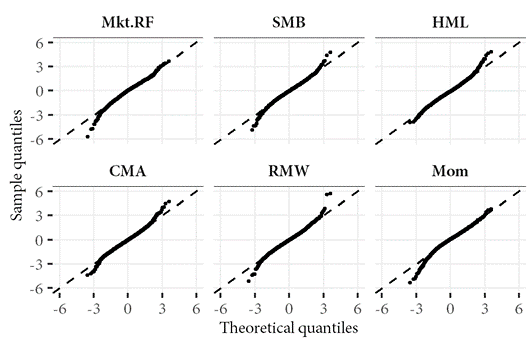
\includegraphics[width = 9cm]{graphics/qq_norm.png}
    \caption{Normal}
  \end{subfigure}
  \\
  \begin{subfigure}{9cm}
    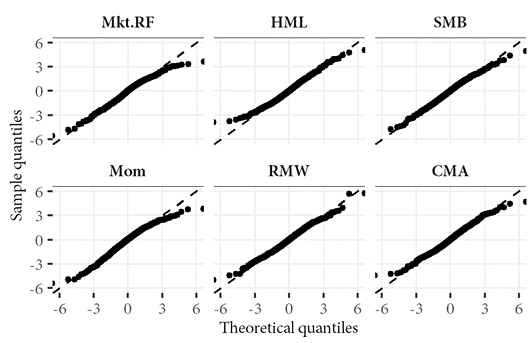
\includegraphics[width = 9cm]{graphics/qq_std.png}
    \caption{Symmetric \emph{t}}
  \end{subfigure}
  \\
  \begin{subfigure}{9cm}
    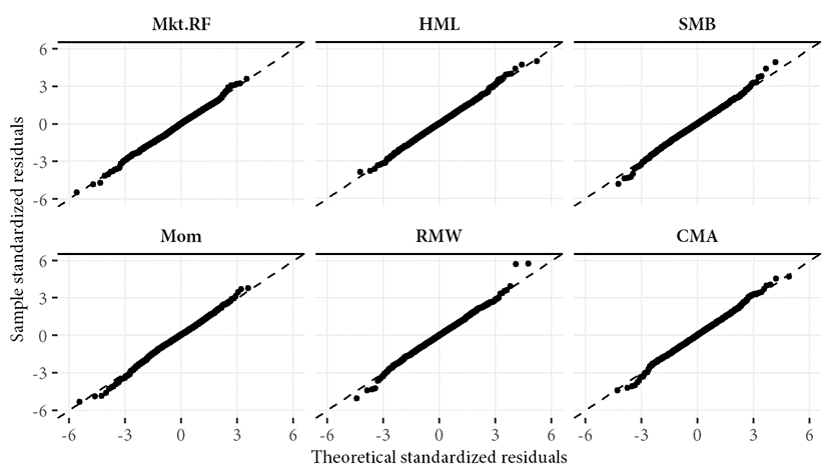
\includegraphics[width = 9cm]{graphics/qq_ghst.png}
    \caption{Asymmetric \emph{t}}
  \end{subfigure}
  \caption{QQ plots of standardized residuals}
  \begin{longcaption}
    Standardized residuals from the best (lowest BIC) ARMA-GARCH model specifications, with normal, symmetric \emph{t} and skewed \emph{t} innovations. Data from the theoretical distribution should line up on the dashed line. Based on weekly data 1963--2016.
  \end{longcaption}
  \label{fig:garch_qq}
\end{figure}

% In the variance equation, all factors exhibit high $\alpha$ and $\beta$ leading to a high variance persistence, between 0.96 and 0.99. Generally, variance persistence, which is related to volatility clustering, tends to be high in financial return series. [WHAT DOES IT MEAN WHY DO I CARE] We note that the zero-cost factor portfolios are no exception. The HML factor has a higher $\alpha$ estimate, indicating that shocks of equal size translate into slightly stronger volatility for HML than for RMW and CMA. RMW, on the other hand, has both the lowest $\alpha$ estimate and the highest $\beta$ estimate, indicating higher persistence and lower sensitivity of volatility to shocks.

% We note that the Mkt.RF factor is, according to our model selection procedure, best fitted by a ARMA(0, 0) mean equation, indicating no predictive power of 1-week lagged returns. Also, in the variance equation, we note that the relatively low $\alpha = 0.037$ sensitivity to shocks is increased considerably by $\eta = 0.181$ in the case of a \emph{negative} shock. Furthermore, the Mom factor stands out with a much higher estimate of $\alpha$ (0.186) than any of the other series (all around 0.10) and a lower $\beta$ (0.793). This means that volatility in the momentum factor is more sensitive than other factor strategies to return shocks and less predictable by past volatility alone. We also note that the Mkt.RF and Mom factors exhibit relatively higher unconditional volatilities (of 0.022 and 0.018) than do other factors (around 0.010).

Many of the estimates of $\gamma_i$, the skewness of the skewed \emph{t} GARCH innovation process, are statistically insignificant. This is also the case for the degree of freedom estimates, $\nu$ for the SMB and Mom models. Although these parameters are not significantly estimated, we believe that including them is essential, as QQ-plots indicate misspecification for the models with normal and symmetric \emph{t} innovations.

% subsection univariate_modeling_of_returns (end)
